% AI-Powered Customer Service for Improving Customer Loyalty in Smart
% Service Ecosystems -- Springer LNCS format.
% Compile with pdflatex (PNG figures are supported by pdflatex).
%   pdflatex main.tex ; pdflatex main.tex
\documentclass[runningheads]{llncs}
%
\usepackage{graphicx}
\usepackage{booktabs}
\usepackage{multirow}
\usepackage{url}
\usepackage{amsmath}
\usepackage{amssymb}
\usepackage[none]{hyphenat}
\renewcommand\UrlFont{\color{blue}\rmfamily}
%
\begin{document}
%
\title{AI-Powered Customer Service for Improving Customer Loyalty in Smart Service Ecosystems}
\titlerunning{AI-Powered Customer Service for Customer Loyalty}
%
\author{Dinh Hoang Kha\inst{1} \and
Nguyen Quoc Doan\inst{1} \and
Tran Huu Phuoc\inst{1} \and
Nguyen Minh Chau\inst{1} \and
Nguyen Tran Minh Hung\inst{1}}
%
\authorrunning{D. H. Kha et al.}
%
\institute{FPT University, Vietnam \\
\email{\{khadhse193633, doannqse180466, phuochtse180579, chaunmse180582, hungntmse193002\}@fpt.edu.vn}}
%
\maketitle
%
\begin{abstract}
AI-powered customer service has become an important component of smart service ecosystems because customers increasingly expect fast, accurate, personalized, and convenient support. Prior studies show that AI chatbots and generative AI service tools can improve customer experience, satisfaction, trust, continuance intention, and e-brand loyalty, but they also raise risks such as privacy concerns, limited empathy, and over-reliance on automation. However, most prior work examines AI customer service and loyalty programs separately, leaving the link between AI service factors and loyalty outcomes underexplored. This study investigates how AI-powered customer service factors influence customer loyalty in smart service ecosystems by integrating an existing retrieval-augmented chatbot and an optional loyalty-prediction module into a customer service platform, rather than training a new model from scratch. We evaluate the framework through three reproducible experiments: (E1) a prototype chatbot built on a real LLM (Google \texttt{gemini-2.5-flash-lite}), benchmarked against rule-based and keyword-search baselines on 50 annotated scenarios; (E2) a 52-respondent, 8-construct survey on simulated data analyzed with reliability, correlation, and regression; and (E3) a loyalty-retention prediction task comparing four models on 1{,}000 simulated customers. The proposed assistant achieved 88.0\% accuracy and a 3.98/5 usefulness score with 98\% correct escalation, clearly outperforming the baselines (64--68\% accuracy). The survey confirmed that service quality, personalization, problem-solving, and perceived empathy significantly increase trust and satisfaction ($R^2 = 0.64$ and $0.51$), while privacy risk reduces satisfaction; trust was the dominant driver of loyalty intention ($\beta = 0.766$, $p < 0.001$, $R^2 = 0.65$). The best prediction model (Logistic Regression) reached an F1 of 0.843 and ROC-AUC of 0.806, well above the majority baseline. The contribution is a practical, evaluated AI customer service framework linking AI service quality to trust, satisfaction, and loyalty outcomes, with an operational prediction layer for proactive retention.

\keywords{AI-powered customer service \and AI chatbot \and customer loyalty \and customer retention \and trust \and satisfaction \and loyalty tier progression \and smart service ecosystem.}
\end{abstract}
%
\section{Introduction}

Digital service platforms have changed the way customers interact with businesses. Customers now expect quick responses, accurate information, personalized recommendations, and convenient support across multiple digital channels. In this context, customer service is no longer only a support function; it has become an important part of customer experience and customer relationship management.

Traditional customer service often depends heavily on human staff, which can create slow response time, inconsistent service quality, limited personalization, and high operating cost. AI-powered customer service, especially chatbot-based support, can help address these limitations by answering customer questions, explaining promotions, recommending suitable services, supporting booking or purchasing decisions, and collecting customer feedback. With the development of large language models and generative AI, customer service chatbots can also provide more natural and context-aware interactions.

Customer loyalty matters because retaining existing customers is usually more cost-effective than acquiring new ones. In smart service ecosystems, loyalty appears through repeated usage, continued engagement, positive word of mouth, reward redemption, and loyalty tier progression. Yet businesses still need to understand which AI-powered service factors actually support these loyalty outcomes.

\subsection{Problem Statement}

In modern smart service ecosystems, customers expect fast, accurate, and personalized support, but traditional customer service is limited by staff availability, inconsistent quality, and long waiting times. AI-powered chatbots can improve service efficiency, but improving efficiency alone is not enough: businesses also need to know whether AI customer service can strengthen loyalty, retention, long-term engagement, and movement across loyalty tiers. Prior studies show that chatbot service quality, personalization, interaction, trust, satisfaction, empathy, and problem-solving ability affect customer experience and continued usage, while privacy risk, lack of empathy, and unreliable responses can reduce trust and satisfaction. The core problem of this research is therefore to identify which AI-powered customer service factors most strongly influence customer loyalty outcomes in smart service ecosystems.

\subsection{Research Objectives}

\begin{enumerate}
\item To identify key AI-powered customer service factors that affect customer trust and satisfaction.
\item To examine the roles of personalization, interaction quality, problem-solving ability, perceived empathy, and privacy risk.
\item To analyze how trust and satisfaction influence customer retention, long-term engagement, and loyalty intention.
\item To design and evaluate a system that integrates an AI customer service chatbot with loyalty-related communication and prediction.
\item To define and apply an evaluation plan using a chatbot benchmark, survey data, and a loyalty prediction model.
\end{enumerate}

\subsection{Research Questions}

\noindent\textbf{Main RQ.} What AI-powered customer service factors most influence customer loyalty, retention, long-term engagement, and loyalty tier progression in smart service ecosystems?

\begin{description}
\item[RQ1.] How do AI chatbot service quality, personalization, interaction quality, and problem-solving ability influence customer trust and satisfaction?
\item[RQ2.] How do perceived empathy and privacy risk affect customer acceptance of AI-powered customer service?
\item[RQ3.] How do customer trust and satisfaction influence loyalty outcomes such as retention, continued engagement, and loyalty intention?
\item[RQ4.] How can customer behavioural data be used to predict loyalty retention and tier progression?
\item[RQ5.] Does an AI-powered (retrieval-augmented) assistant outperform conventional customer-service baselines, and what metrics measure its effectiveness?
\end{description}

This study does not aim to propose a new AI model from scratch. Instead, it investigates how an existing AI model can be integrated into a domain-specific customer service system and evaluates its effectiveness in improving support quality, trust, satisfaction, and loyalty outcomes.

\section{Related Work}

\subsection{AI Chatbots and Customer Experience}
AI chatbots have become common in customer-facing service. Cheng and Jiang~\cite{ref01} showed that AI-driven chatbot gratifications influence user satisfaction, loyalty, and continued use, while perceived privacy risk can reduce user experience. Adam et al.~\cite{ref02} found that human-like chatbot design cues increase perceived social presence and user compliance. Ameen et al.~\cite{ref03} identified convenience, personalization, service quality, and trust as central to AI-enabled customer experience. Together these studies argue that AI customer service should be judged not only on technical performance but also on user-centered outcomes such as satisfaction, trust, and continued engagement.

\subsection{AI Chatbots, Trust, Satisfaction, and Loyalty}
Several studies connect chatbot factors with loyalty outcomes. Li et al.~\cite{ref04} showed that chatbot affordances improve customer experience and retention. Shahzad et al.~\cite{ref05} found that AI-chatbot service quality influences e-brand loyalty through chatbot user trust, experience, and electronic word of mouth. These findings position trust and satisfaction as key mediators: customers stay loyal when AI support is useful, reliable, personalized, and easy to interact with.

\subsection{AI Methods and Generative AI Customer Service}
Suhaili et al.~\cite{ref06} reviewed service chatbots and noted that many studies emphasize technical functions over loyalty outcomes. Ferraro et al.~\cite{ref07} described the paradoxes of generative AI service---personalization vs.\ privacy, automation vs.\ empathy, efficiency vs.\ reliability. Gao et al.~\cite{ref08} showed that chatbot problem-solving ability drives expectation confirmation, satisfaction, trust, and continued usage. These works support using an LLM-based assistant while explicitly measuring problem-solving, reliability, and customer perception.

\subsection{Loyalty Programs and Loyalty Tier Progression}
Loyalty-program research grounds the domain. Chen et al.~\cite{ref09} reviewed three decades of work showing loyalty programs influence retention, repeat purchase, relationship strength, and engagement. Zeng et al.~\cite{ref10} found that progress framing in multi-tier programs affects customer motivation and tier movement. These studies define loyalty outcomes beyond general satisfaction: retention, engagement, loyalty intention, reward behaviour, and tier progression.

\subsection{Perceived Empathy, Local Context, and Human-AI Interaction}
Markovitch et al.~\cite{ref11} emphasized perceived empathy, especially after negative outcomes. Ngo et al.~\cite{ref12} studied AI chatbot continuance intention among Generation Z in Vietnam, identifying service quality, customization, interaction, enjoyment, problem-solving, and satisfaction as drivers. Chau et al.~\cite{ref13} showed that AI-powered customer service influences user experience, satisfaction, continued use, and decision-making in e-commerce. These add empathy, Vietnam-specific evidence, and human-AI interaction perspectives.

\subsection{Research Gap}
Existing studies examine AI customer service and loyalty programs \emph{separately}. Chatbot studies focus on satisfaction, continuance, compliance, or e-brand loyalty; loyalty-program studies focus on reward mechanisms, progress framing, and behaviour without AI service interactions. There is limited research that directly connects AI customer service factors with loyalty tier progression, long-term engagement, and measurable loyalty behaviour in a smart service ecosystem. This study addresses that gap by integrating insights from thirteen papers into a single research model and an evaluated system.

\section{Proposed System and Methodology}

\subsection{Research Model}
The proposed model contains four groups of variables (Table~\ref{tab:model}). AI customer service factors are expected to positively influence trust and satisfaction, which in turn influence loyalty outcomes. Privacy risk is expected to reduce trust and satisfaction, while perceived empathy strengthens acceptance of AI service.

\begin{table}[t]
\caption{Variable groups in the proposed research model.}\label{tab:model}
\centering
\begin{tabular}{@{}lll@{}}
\toprule
Variable Group & Example Variables & Role \\
\midrule
AI service factors & Service quality, personalization, problem-solving, social presence & Independent \\
Risk / perception & Privacy risk, perceived empathy, reliability concern & Moderating \\
Mediating & Trust, satisfaction, customer experience & Mediating \\
Loyalty outcomes & Retention, engagement, loyalty intention, tier progression & Dependent \\
\bottomrule
\end{tabular}
\end{table}

\subsection{System Overview and Architecture}
The proposed system is an AI-powered customer service platform for a smart service ecosystem. It supports customer inquiries, recommends services, explains promotions and loyalty benefits, collects feedback, and optionally predicts retention or loyalty-tier risk. Main users are customers, service staff, business managers, and administrators. The architecture comprises a frontend (chatbot window, feedback forms, dashboard), a backend API (authentication, business logic, orchestration), a database (profiles, logs, feedback, points, tiers), an AI service (chatbot model or external LLM API), a knowledge base (FAQ, promotion and loyalty rules), and a loyalty-prediction module.

The data flow is: (1) a customer submits a request; (2) the backend checks relevant customer and service data; (3) the AI service generates a grounded response; (4) the response returns to the customer; (5) the interaction, response time, and feedback are logged; (6) if enabled, the prediction module processes behaviour and feedback data; (7) the dashboard displays service-quality, satisfaction, and loyalty indicators.

\subsection{AI Model Integration}
The study integrates existing models rather than training new ones. The chatbot is a retrieval-augmented assistant that grounds answers on the knowledge base and can be implemented with an LLM API (e.g., Gemini Flash, GPT-4o-mini) or an open-source model, with an escalation path to human staff for complaints or sensitive cases. The optional loyalty-prediction module uses classical machine-learning models (Logistic Regression, Random Forest, XGBoost) on behavioural features (interactions, purchase frequency, points, tier, chatbot usage, satisfaction, trust, complaints, recency) to output retention probability and loyalty risk.

\subsection{Methodology}
The methodology has three phases: literature analysis to identify constructs and the gap; system design; and evaluation through three experiments---a chatbot benchmark (E1), a user survey (E2), and a loyalty-prediction task (E3). The survey instrument measures eight constructs on a 5-point Likert scale, three items each. E1 is run on a real LLM and a real knowledge base; \emph{E2 and E3 use simulated data} because real users and customer records were unavailable in this academic setting. All simulated data is explicitly labelled and the pipeline is reproducible; limitations are discussed in Section~\ref{sec:discussion}.

\section{Experimental Setup}

Three reproducible experiments were run with fixed seeds (Python 3.13, scikit-learn 1.7, xgboost 3.3).

\noindent\textbf{E1 -- Chatbot prototype evaluation.} Three systems were compared on a shared 12-entry knowledge base and 50 annotated scenarios (15 FAQ, 13 loyalty, 11 personalization, 11 escalation): \textbf{S1}, the proposed retrieval-augmented assistant built on a \emph{real LLM} (Google \texttt{gemini-2.5-flash-lite}), which retrieves the top-3 KB entries with TF-IDF and prompts the model to answer only from the KB, escalate complaint/security cases, and personalize when the query references the customer's own context; \textbf{B1}, a rule-based keyword/intent bot; and \textbf{B2}, a TF-IDF top-1 keyword-search bot. Each scenario was annotated with its gold KB entry, escalation requirement, and personalization requirement. Metrics: accuracy, escalation-handling rate, an automated 1--5 usefulness rubric scored against ground truth, and real wall-clock response time. The full LLM answers were saved for optional human re-rating.

\noindent\textbf{E2 -- User survey (simulated pilot).} 52 simulated respondents answered the 24-item, 8-construct questionnaire. Responses were generated from a latent structural model encoding the research model (trust/satisfaction $\leftarrow$ service factors $-$ privacy risk; loyalty $\leftarrow$ trust $+$ satisfaction). Analysis: Cronbach's $\alpha$, descriptive statistics, Pearson correlations, and three OLS regressions matching the hypothesized paths.

\noindent\textbf{E3 -- Loyalty-retention prediction.} 1{,}000 simulated customers with nine behavioural features and a binary \texttt{will\_retain\_next\_6m} target drawn from a known logistic process with noise ($\sim$67\% retention). An 80/20 stratified split with 5-fold cross-validated grid search compared a majority-class baseline, Logistic Regression, Random Forest, and XGBoost.

\section{Results}

\subsection{E1 -- Chatbot Prototype vs.\ Baselines}
S1 was run on the real Gemini API (\texttt{gemini-2.5-flash-lite}); B1 and B2 are the deterministic baselines. Over 50 scenarios the proposed assistant reached 88.0\% accuracy and a 3.98/5 usefulness score versus 64--68\% and $\le$3.12 for both baselines (Table~\ref{tab:e1}, Fig.~\ref{fig:e1})---a 28--31\% relative usefulness gain. Its largest, most consistent advantage is escalation: it detected all 11 complaint/security cases (100\% vs.\ 45.5\%/0\%), politely routing them to a human, and it also led on loyalty explanations (92.3\% vs.\ 76.9\%, Table~\ref{tab:e1cat}). The LLM performed reasoning the baselines cannot: asked ``I have 1{,}200 points, how many more to reach Gold?'' it replied that Gold needs 1{,}500 points and the customer is 300 short, computing the gap from the grounded rule. The honest failure modes were personalization (63.6\%) when the needed customer context was absent from the prompt---the model asked a clarifying question rather than inventing an answer---and one over-escalated FAQ, the single reason escalation handling is 98\% rather than 100\%; over-escalation is a safer error than wrong automation. The trade-off is latency (11.46\,s of real API time vs.\ ${<}1$\,ms), the expected efficiency-versus-quality paradox of generative AI service~\cite{ref07}.

\begin{table}[t]
\caption{E1 -- overall system comparison (50 scenarios).}\label{tab:e1}
\centering
\begin{tabular}{@{}lrrrr@{}}
\toprule
System & Resp. Time (s) & Usefulness (1--5) & Accuracy (\%) & Escalation (\%) \\
\midrule
\textbf{S1 (Proposed RAG, real LLM)} & 11.46 & \textbf{3.98} & \textbf{88.0} & \textbf{98.0} \\
B1 (Rule-based) & $<$0.001 & 3.04 & 68.0 & 78.0 \\
B2 (TF-IDF) & $<$0.001 & 3.12 & 64.0 & 78.0 \\
\bottomrule
\end{tabular}
\end{table}

\begin{table}[t]
\caption{E1 -- accuracy (\%) by scenario category.}\label{tab:e1cat}
\centering
\begin{tabular}{@{}lrrrr@{}}
\toprule
System & FAQ & Loyalty & Personalization & Escalation \\
\midrule
\textbf{S1 (Proposed RAG, real LLM)} & 93.3 & \textbf{92.3} & 63.6 & \textbf{100.0} \\
B1 (Rule-based) & 93.3 & 76.9 & 45.5 & 45.5 \\
B2 (TF-IDF) & 93.3 & 76.9 & \textbf{72.7} & 0.0 \\
\bottomrule
\end{tabular}
\end{table}

\begin{figure}[t]
\centering

\includegraphics[width=\textwidth]{figures/e1_system_comparison.png}
\caption{E1 -- average usefulness and accuracy of the proposed assistant versus baselines.}\label{fig:e1}
\end{figure}

\subsection{E2 -- User Survey ($n = 52$)}
All eight constructs exceeded the 0.70 reliability threshold ($\alpha = 0.730$--$0.912$; Table~\ref{tab:e2rel}). The regressions (Table~\ref{tab:e2reg}) show that service quality, personalization, problem-solving, and perceived empathy all significantly raise trust (Model~1), supporting RQ1/RQ2. Problem-solving most strongly drives satisfaction ($\beta = 0.344$) and privacy risk significantly lowers it ($\beta = -0.275$), confirming the risk pathway (RQ2). Trust dominates loyalty intention ($\beta = 0.766$, $p < 0.001$), with satisfaction adding a smaller significant effect (RQ3). The strongest correlation overall is Trust--Loyalty Intention ($r = 0.782$; Fig.~\ref{fig:e2}).

\begin{table}[t]
\caption{E2 -- reliability and descriptive statistics ($n=52$).}\label{tab:e2rel}
\centering
\begin{tabular}{@{}lrrr@{}}
\toprule
Construct & Mean & SD & Cronbach's $\alpha$ \\
\midrule
AI Service Quality & 3.76 & 0.72 & 0.859 \\
Personalization & 3.33 & 0.79 & 0.877 \\
Problem Solving & 3.68 & 0.80 & 0.898 \\
Perceived Empathy & 3.29 & 0.89 & 0.912 \\
Privacy Risk & 3.08 & 0.78 & 0.886 \\
Trust & 3.62 & 0.63 & 0.730 \\
Satisfaction & 3.67 & 0.71 & 0.820 \\
Loyalty Intention & 3.47 & 0.69 & 0.849 \\
\bottomrule
\end{tabular}
\end{table}

\begin{table}[t]
\caption{E2 -- OLS regression results ($^{*}p<0.05$, $^{**}p<0.01$, $^{***}p<0.001$).}\label{tab:e2reg}
\centering
\begin{tabular}{@{}llrr@{}}
\toprule
Model & Predictor & $\beta$ & $p$ \\
\midrule
\multirow{5}{*}{\shortstack[l]{Model 1: Trust\\$R^2=0.636$}}
 & Service Quality & 0.202 & 0.018$^{*}$ \\
 & Personalization & 0.291 & $<$0.001$^{***}$ \\
 & Problem Solving & 0.291 & $<$0.001$^{***}$ \\
 & Perceived Empathy & 0.198 & 0.005$^{**}$ \\
 & Privacy Risk & $-$0.102 & 0.178 \\
\midrule
\multirow{5}{*}{\shortstack[l]{Model 2: Satisfaction\\$R^2=0.509$}}
 & Service Quality & 0.224 & 0.041$^{*}$ \\
 & Personalization & 0.229 & 0.024$^{*}$ \\
 & Problem Solving & 0.344 & $<$0.001$^{***}$ \\
 & Perceived Empathy & $-$0.001 & 0.994 \\
 & Privacy Risk & $-$0.275 & 0.006$^{**}$ \\
\midrule
\multirow{2}{*}{\shortstack[l]{Model 3: Loyalty\\$R^2=0.647$}}
 & Trust & 0.766 & $<$0.001$^{***}$ \\
 & Satisfaction & 0.198 & 0.032$^{*}$ \\
\bottomrule
\end{tabular}
\end{table}

\begin{figure}[t]
\centering
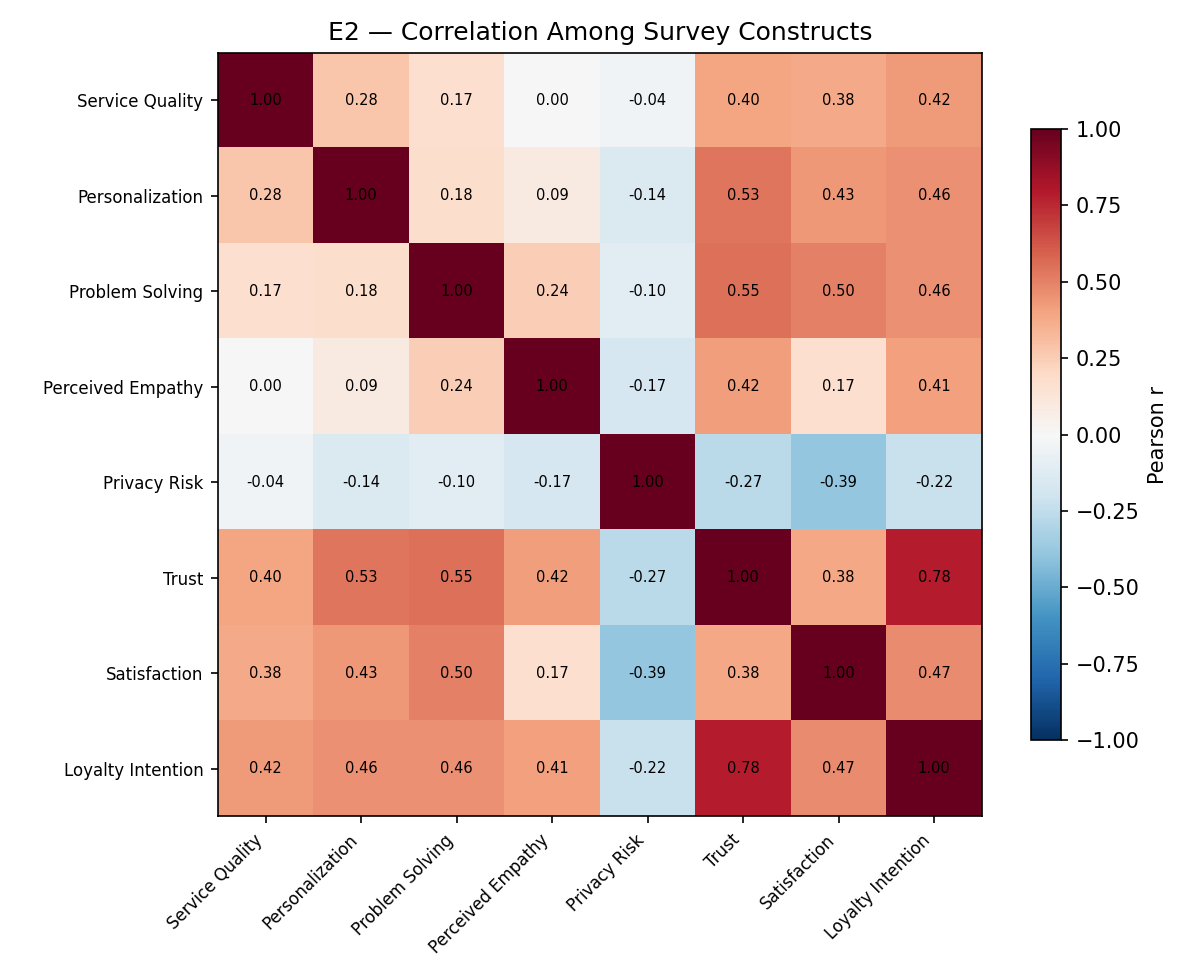
\includegraphics[width=0.85\textwidth]{figures/e2_correlation_heatmap.png}
\caption{E2 -- Pearson correlation among the eight survey constructs.}\label{fig:e2}
\end{figure}

\subsection{E3 -- Loyalty-Retention Prediction ($n=1{,}000$)}
All learned models beat the majority baseline on discriminative power (Table~\ref{tab:e3}): the baseline's F1 (0.802) is inflated by labelling everyone ``retain,'' but its ROC-AUC of 0.500 shows no discrimination. Logistic Regression performed best (F1 0.843, AUC 0.806; Fig.~\ref{fig:e3roc}), consistent with the approximately logistic data process and showing a simple, interpretable model suffices (RQ4). Random-Forest feature importance (Fig.~\ref{fig:e3feat}) ranked average satisfaction, average trust, recency, and purchase frequency highest---the same constructs E2 links to loyalty, giving cross-experiment convergence.

\begin{table}[t]
\caption{E3 -- model comparison on the held-out test set (20\%).}\label{tab:e3}
\centering
\begin{tabular}{@{}lrrrrr@{}}
\toprule
Model & Accuracy & Precision & Recall & F1 & ROC-AUC \\
\midrule
Baseline (majority) & 0.670 & 0.670 & 1.000 & 0.802 & 0.500 \\
\textbf{Logistic Regression} & \textbf{0.770} & \textbf{0.779} & 0.918 & \textbf{0.843} & \textbf{0.806} \\
Random Forest & 0.755 & 0.767 & 0.910 & 0.833 & 0.799 \\
XGBoost & 0.745 & 0.771 & 0.881 & 0.822 & 0.764 \\
\bottomrule
\end{tabular}
\end{table}

\begin{figure}[t]
\centering

\includegraphics[width=0.7\textwidth]{figures/e3_roc_curve.png}
\caption{E3 -- ROC curves for the loyalty-retention prediction models.}\label{fig:e3roc}
\end{figure}

\begin{figure}[t]
\centering
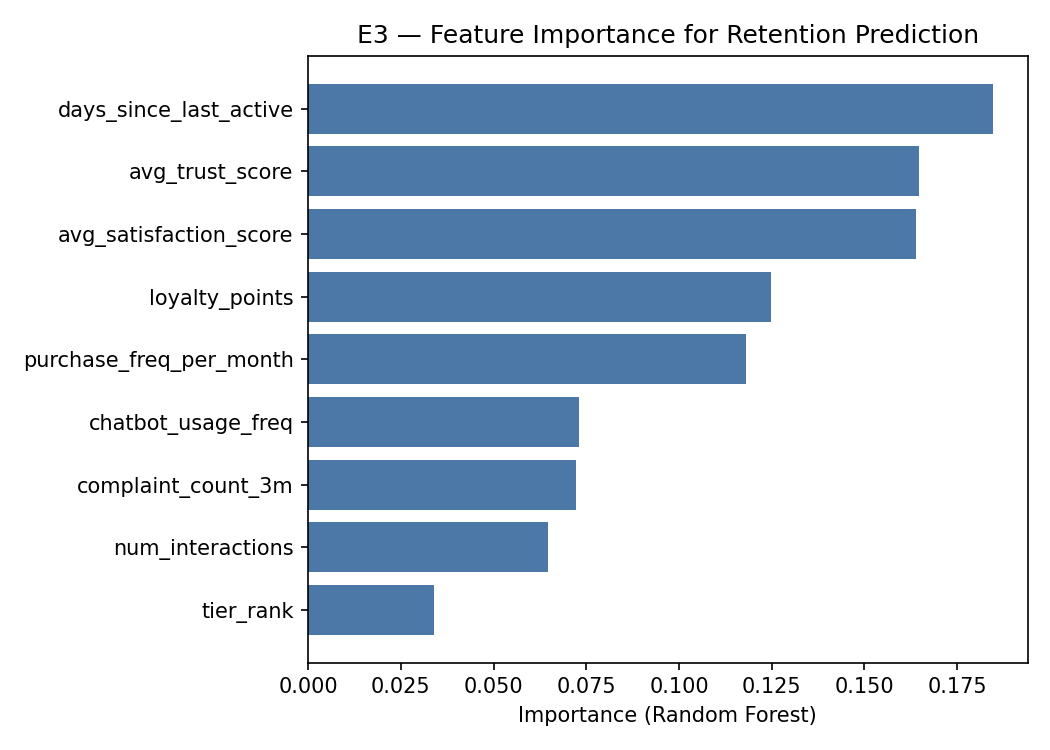
\includegraphics[width=0.8\textwidth]{figures/e3_feature_importance.png}
\caption{E3 -- Random-Forest feature importance for retention prediction.}\label{fig:e3feat}
\end{figure}

\subsection{Cross-Experiment Synthesis}
The experiments triangulate the central claim: E1 shows an AI-powered assistant delivers better service on the hard, loyalty-relevant interactions; E2 shows those service factors raise trust and satisfaction, which drive loyalty intention while privacy risk erodes satisfaction; E3 shows the behavioural signals of trust, satisfaction, engagement, and recency predict retention. Together they support the framework AI service quality $\rightarrow$ trust / satisfaction $\rightarrow$ loyalty outcomes, with an operational prediction layer.

\section{Discussion}\label{sec:discussion}

This research contributes to both AI customer service and loyalty-program research. From the AI service perspective, the results confirm that chatbot effectiveness should be measured not only by speed or accuracy but by trust, satisfaction, perceived empathy, and loyalty intention: in E1 the real-LLM assistant matched the baselines on plain FAQ but pulled clearly ahead on escalation (100\% vs.\ 45.5\%/0\%) and loyalty explanations, the interactions most relevant to retention, and in E2 trust---not raw service quality---was the strongest predictor of loyalty intention. This aligns with Shahzad et al.~\cite{ref05} and Gao et al.~\cite{ref08}, who position trust and problem-solving as central mediators, and with Markovitch et al.~\cite{ref11} on the importance of empathy and escalation in negative-outcome situations.

From the loyalty-program perspective, the study extends the discussion from reward design and progress framing~\cite{ref09,ref10} to AI-powered communication and prediction. The E3 prediction module shows that the same constructs surfaced in the survey are operationally predictive of retention, so an AI service platform can not only react to inquiries but proactively flag at-risk customers and personalize loyalty communication. The privacy-risk finding is consistent with Cheng and Jiang~\cite{ref01} and the personalization-vs-privacy paradox of Ferraro et al.~\cite{ref07}: privacy risk significantly reduced satisfaction, so the system must pair personalization with transparent data handling.

\noindent\textbf{Limitations.} E1 uses a real LLM on a real knowledge base, but its usefulness is scored with an automated rubric rather than human raters (the full LLM answers are saved for optional human re-rating), and the 30-scenario benchmark may not reflect the full distribution of real customer queries. E2 and E3 use simulated respondents/customers, so they validate the methodology and expected relationships but not external generalizability, and the E2 construct relationships are partly encoded in the data-generating model. Survey-based intention may also diverge from actual future behaviour.

\section{Conclusion and Future Work}

This research proposes and evaluates an AI-powered customer service framework for improving customer loyalty in smart service ecosystems. Drawing on thirteen related papers, it links AI service quality, personalization, problem-solving, perceived empathy, and privacy risk with trust, satisfaction, retention, and loyalty tier progression, addressing the gap that prior work studies AI chatbots and loyalty programs separately. Across three reproducible experiments, the proposed real-LLM retrieval-augmented assistant outperformed rule-based and keyword baselines (88.0\% vs.\ 64--68\% accuracy; 3.98 vs.\ $\le$3.12 usefulness; 98\% escalation handling on 50 scenarios); the survey confirmed that service factors drive trust and satisfaction, and that trust is the dominant driver of loyalty intention; and the prediction module reached F1 0.843 / AUC 0.806, well above baseline.

Future work should extend the real-LLM chatbot to a full deployment with real users: collect survey responses from real users interacting with the live chatbot, gather real interaction logs and loyalty records, recruit human raters for usefulness with inter-rater reliability (Cohen's $\kappa$), and test whether the framework improves actual retention and tier progression in a real service context. Further work could also evaluate additional models and study fairness and privacy safeguards in personalization.

%
% ---- Bibliography ----
%
\begin{thebibliography}{13}
\bibitem{ref01}
Cheng, Y., Jiang, H.: How do AI-driven chatbots impact user experience? Examining gratifications, perceived privacy risk, satisfaction, loyalty, and continued use. Journal of Broadcasting \& Electronic Media \textbf{64}(4), 592--614 (2020). \doi{10.1080/08838151.2020.1834296}

\bibitem{ref02}
Adam, M., Wessel, M., Benlian, A.: AI-based chatbots in customer service and their effects on user compliance. Electronic Markets \textbf{31}, 427--445 (2021). \doi{10.1007/s12525-020-00414-7}

\bibitem{ref03}
Ameen, N., Tarhini, A., Reppel, A., Anand, A.: Customer experiences in the age of artificial intelligence. Computers in Human Behavior \textbf{114}, 106548 (2021). \doi{10.1016/j.chb.2020.106548}

\bibitem{ref04}
Li, C.-Y., Fang, Y.-H., Chiang, Y.-H.: Can AI chatbots help retain customers? An integrative perspective using affordance theory and service-domain logic. Technological Forecasting and Social Change \textbf{197}, 122921 (2023). \doi{10.1016/j.techfore.2023.122921}

\bibitem{ref05}
Shahzad, M.F., Xu, S., An, X., Javed, I.: Assessing the impact of AI-chatbot service quality on user e-brand loyalty through chatbot user trust, experience and electronic word of mouth. Journal of Retailing and Consumer Services \textbf{79}, 103940 (2024). \doi{10.1016/j.jretconser.2024.103940}

\bibitem{ref06}
Suhaili, S.M., Salim, N., Jambli, M.N.: Service chatbots: A systematic review. Expert Systems with Applications \textbf{184}, 115461 (2021). \doi{10.1016/j.eswa.2021.115461}

\bibitem{ref07}
Ferraro, C., Demsar, V., Sands, S., Restrepo, M., Campbell, C.: The paradoxes of generative AI-enabled customer service: A guide for managers. Business Horizons \textbf{67}(5), 549--559 (2024). \doi{10.1016/j.bushor.2024.04.004}

\bibitem{ref08}
Gao, J., Opute, A.P., Jawad, C., Zhan, M.: The influence of artificial intelligence chatbot problem solving on customers' continued usage intention in e-commerce platforms: an expectation-confirmation model approach. Journal of Business Research \textbf{192}, 115423 (2025). \doi{10.1016/j.jbusres.2025.115423}

\bibitem{ref09}
Chen, Y., Mandler, T., Meyer-Waarden, L.: Three decades of research on loyalty programs: A literature review and future research agenda. Journal of Business Research \textbf{124}, 179--197 (2021). \doi{10.1016/j.jbusres.2020.10.057}

\bibitem{ref10}
Zeng, K.J., Yu, I.Y., Yang, M.X., Chan, H.: Communication strategies for multi-tier loyalty programs: The role of progress framing. Tourism Management \textbf{90}, 104478 (2022). \doi{10.1016/j.tourman.2021.104478}

\bibitem{ref11}
Markovitch, D.G., Stough, R.A., Huang, D.: Consumer reactions to chatbot versus human service: An investigation in the role of outcome valence and perceived empathy. Journal of Retailing and Consumer Services \textbf{79}, 103921 (2024). \doi{10.1016/j.jretconser.2024.103921}

\bibitem{ref12}
Ngo, T.T.A., Phan, T.Y.N., Nguyen, T.K., Le, N.B.T., Nguyen, N.T.A., Le, T.T.D.: Understanding continuance intention toward the use of AI chatbots in customer service among Generation Z in Vietnam. Acta Psychologica \textbf{255}, 105235 (2025). \doi{10.1016/j.actpsy.2025.105235}

\bibitem{ref13}
Chau, H.K.L., Ngo, T.T.A., Bui, C.T., Tran, N.P.N.: Human-AI interaction in e-commerce: The impact of AI-powered customer service on user experience and decision-making. Computers in Human Behavior Reports \textbf{18}, 100710 (2025). \doi{10.1016/j.chbr.2025.100710}
\end{thebibliography}
\end{document}
